To empirically evaluate Cerebro, we conduct experiments using five open source, Google
App Engine applications.

\begin{description}
\item[StudentInfo] RESTful (JAX-RS) application for managing
students of a class (adding, removing, and listing student information).
\item[ServerHealth] Monitors, computes, and reports statistics for server
uptime for a given web URL.
\item[SocialMapper] A simple social networking application with APIs for
adding users and comments.
\item[StockTrader] A stock trading application that
provides APIs for adding users, registering companies, buying and selling
stocks among users. 
\item[Rooms] A hotel booking application with APIs
for registering hotels and querying available rooms.
\end{description}

These web APIs use the datastore
cloud SDK interface extensively. The Rooms web API also uses the
memcache interface. We focus on these two interfaces exclusively in this
study. We execute these applications in the Google App Engine public cloud 
(SDK v1.9.17)
and in an AppScale (v2.0) private cloud.  We instrument the programs to collect
execution time statistics for verification purposes only 
(the instrumentation data is not used to predict
the SLAs).  The AppScale private cloud used for testing was
hosted using four ``m3.2xlarge'' virtual machines running on a private
Eucalyptus~\cite{eucalyptus09} cloud.

%We instrument each of the five sample applications to measure the 
%time taken by their web APIs to execute the
%enclosed code. This is done by adding some extra Java code to each of the web APIs exposed by the sample applications.
%We ensure that the instrumentation does not alter the original web API code in anyway (i.e. the original algorithms, control flow
%and data flow are not impacted by the instrumentation). Then for each application we also
%implement a mechanism to output the measured execution times, so an external client can query and collect the execution
%times of the web APIs.

%We carry out each of our tests in two separate environments -- Google App Engine public cloud, and
%the AppScale private cloud. 
%The AppScale private cloud used for testing was powered by four m3.2xlarge virtual machines 
%running on a private Eucalyptus~\cite{eucalyptus09} cluster.

We first report the time required for Cerebro to perform its analysis and SLA prediction.
Across web APIs, Cerebro takes $10.00$ seconds on average, with a 
maximum time of $14.25$ seconds for StudentInfo.
These times include that taken
by the static analyzer to analyze all the web API operations
and the time taken by QBETS to make predictions. For these results, the length of 
the time series collected by PaaS monitoring agent is $1528$ data points ($25.5$ hours of monitoring data). Since the QBETS analysis time depends on the length of the input time series, 
we also measured the time for 2 weeks of monitoring data ($19322$ data points) to provide
some insight into the overhead of SLA prediction.  Even in this case, Cerebro
requires only $574.05$ seconds ($9.6$ minutes).

\subsection{Correctness of Predictions}
\label{sec:correctness}

We first evaluate the correctness of Cerebro predictions.  A set of
predictions is \textit{correct} if the \textit{fraction} of measured 
response time values that fall below the Cerebro prediction is greater than 
or equal to the SLA target probability. 
For example, if the SLA probability is $0.95$ (i.e. $p=95$ in QBETS) for
a specific web API, then the Cerebro predictions are correct if at least
$95\%$ of the response times measured for the web API are smaller than their
corresponding Cerebro predictions. 

We benchmark each web API for a period of 15 to 20 hours.  During this time we
run a remote HTTP client that makes requests to the web APIs once every
minute.  The application instrumentation measures and records the response
time of the API operation for each request (i.e. within the application).
Concurrently and within the same PaaS system, we execute the Cerebro
PaaS monitoring agent which is an independently hosted application within the
cloud that benchmarks each SDK operation once every minute.

Cerebro predicts the web API execution times using only the cloud SDK
benchmarking data collected by Cerebro's PaaS monitoring agent. 
We configure Cerebro to predict an
upper bound for the $95^{th}$ percentile of the web API response time, with an
upper confidence of $0.01$. 

QBETS generates a prediction for \textit{every} value in the input time series 
(one per minute).  Cerebro reports the last one as the SLA prediction to the
user or PaaS administrator in production.  However, having per-minute predictions 
enables us to compare these predictions against actual web API execution
times measured during the same time period to evaluate Cerebro correctness. 
More specifically, we
associate with each measurement the prediction from the prediction time series
that most nearly precedes it in time.  The correctness fraction is computed
from a sample of $1000$ prediction-measurement pairs.

%align the sequence of predictions with the time series of actual
%execution time measurements, and check whether each prediction is equal to or
%higher than the corresponding measurement. We consider a sequence of 1000
%consecutive predictions and 1000 consecutive API execution time measurements,
%and compute the percentage of measurements that are less than or equal to the
%predicted values (a metric that we refer to as \textit{percentage accuracy}).

\begin{figure}
\centering
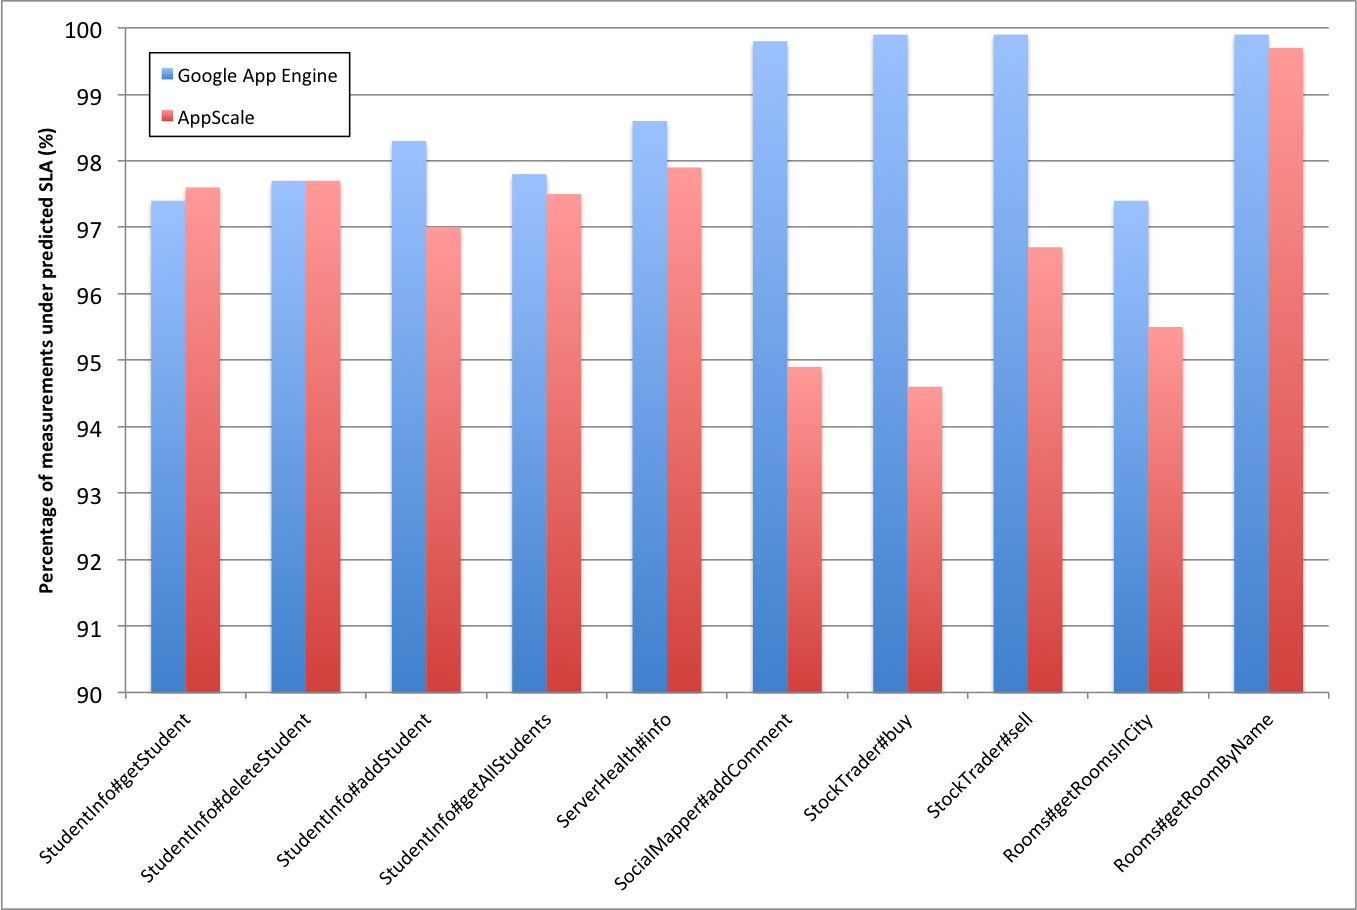
\includegraphics[scale=0.35]{accuracy_summary}
\caption{Cerebro Correctness Percentage in Google App Engine and AppScale cloud platforms.}
\label{fig:accuracy_summary}
\vspace{-0.2in}
\end{figure}

Figure~\ref{fig:accuracy_summary} shows the final results of this experiment.
Each of the columns in Figure~\ref{fig:accuracy_summary} corresponds 
to a single web API operation in 
one of the sample applications. The columns are labeled in the 
form of \textit{ApplicationName\#OperationName}, a convention 
we will continue to use in the rest of the paper. %To maintain clarity in the figures we do not 
%illustrate the results for all web API operations in the sample applications. Instead we present the results for a selected set of 
%web API operations covering all five sample applications. We note that other web API operations we tested also produce
%very similar results.

Since we are using Cerebro to predict the $95^{th}$ percentile of the API
response times, Cerebro's predictions are correct when at 
least $95\%$ of the measured response times are
less than their corresponding predicted upper bounds. According to
Figure~\ref{fig:accuracy_summary}, Cerebro achieves this goal for all the
applications in both cloud environments. 
%The lowest percentage accuracy observed in our tests is 94.6\% (in the case
%of StockTrader\#buy on AppScale), which is also very close to the target of
%95\%.  Such minor lapses below 95\% are acceptable anyway, since we expect
%percentage accuracy value to be gently fluctuating around some average value
%over time (a phenomenon that will be explained in our later results).
%Overall, this result shows us that Cerebro produces highly accurate SLA
%predictions for a variety of applications running on two very different cloud
%platforms.

The web API operations illustrated in Figure~\ref{fig:accuracy_summary} cover
a wide spectrum of scenarios that may be encountered in real world.
StudentInfo\#getStudent and StudentInfo\#addStudent are by far the simplest
operations in the mix. They invoke a single cloud SDK operation each, and
perform a simple datastore read and a simple datastore write respectively. As
per our survey results, these alone cover a significant portion of the web
APIs developed for the App Engine and AppScale cloud platforms (1 path through
the code, and 1 cloud SDK call).  The StudentInfo\#deleteStudent operation
makes two cloud SDK operations in sequence, whereas
StudentInfo\#getAllStudents performs an iterative datastore read.  In our
experiment with StudentInfo\#getAllStudents, we had the datastore preloaded
with $1000$ student records, and Cerebro was configured to use a maximum entity
count of $1000$ when making predictions.

ServerHealth\#info invokes the same cloud SDK operation three times in
sequence. Both StockTrader\#buy and StockTrader\#sell have multiple paths
through the application 
(due to branching), thus causing Cerebro to make multiple
sequences of predictions -- one sequence per path. The results shown in
Figure~\ref{fig:accuracy_summary} are for the longest paths which consist of
seven cloud SDK invocations each. According to our survey, $99.8\%$ of the
execution paths found in Google App Engine applications have seven or 
fewer cloud SDK
calls in them. Therefore we believe that the StockTrader web API
represents an important upper bound case. 

Rooms\#getRoomByName
invokes two different cloud SDK interfaces, namely datastore and memcache.
Rooms\#get\-AllRooms is another operation that consists of an iterative
datastore read. In this case, we had the datastore preloaded with $10$ entities,
and Cerebro was configured to use a maximum entity count of $10$. 
%It is indeed encouraging to see how Cerebro manages to produce highly accurate predictions
%for such a wide range 
%of web API implementations and runtime scenarios on two cloud platforms.

\subsection{Tightness of Predictions}

In this section we discuss the tightness of the predictions generated by Cerebro. 
Tightness is a measure of how closely the predictions
bound the actual response times of the web APIs. 
Note that it is possible to perfectly achieve the correctness goal
by simply predicting overly large values for web API response times. For example, if Cerebro were to
predict a response time of several years for exactly $95\%$ of the web API
invocations and zero for the others, it would likely
achieve a correctness percentage of $95\%$.  From a practical perspective,
however, such an extreme upper bound is not useful as the basis for an SLA. 
%This parameter is just as important as the percentage of measurements that fall under the predicted SLA values. 
%Note that Cerebro can achieve a very high percentage accuracy level by simply generating a 
%sequence of large predictions. But such results will obviously be of very little use to the API
%developers. For the predictions to be useful and meaningful, they should be very close to the actual response times of the web APIs.

\begin{figure}
\centering
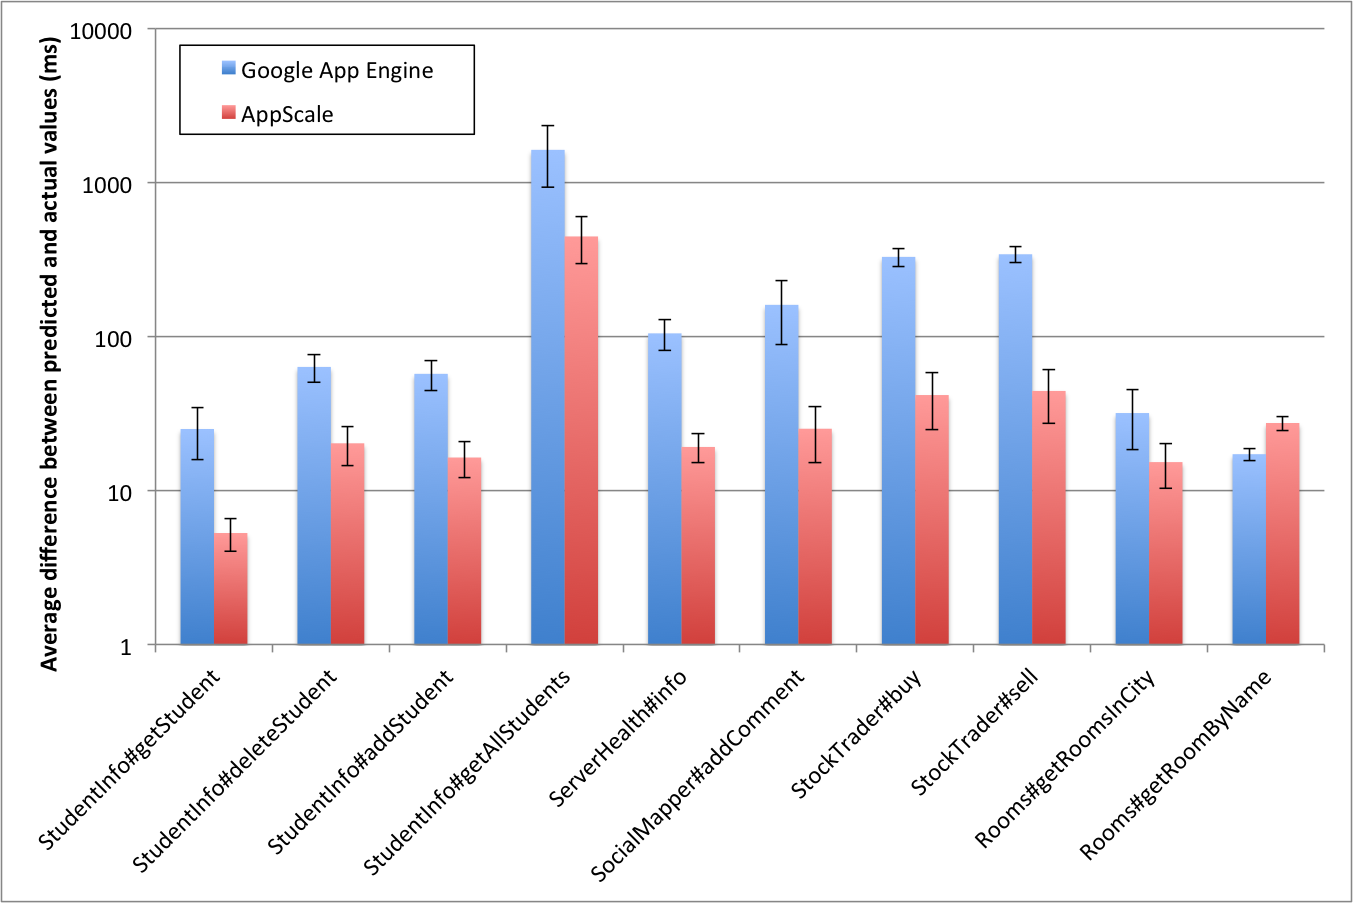
\includegraphics[scale=0.35]{diff_summary}
\caption{Average difference between predictions and actual response times in
Google App Engine and AppScale. The y-axis is in log scale.}
\label{fig:diff_summary}
\vspace{-0.2in}
\end{figure}

Figure~\ref{fig:diff_summary} depicts the average difference between predicted
response time bounds and actual response times for
our sample web APIs when running in the App Engine and AppScale clouds. 
These results were obtained considering a sequence of $1000$ 
consecutive predictions (of $95^{th}$ percentile) and the averages are
computed only for correct predictions (i.e. ones above their corresponding
measurements).
%Within these prediction sequences only the cases 
%where the predicted value was larger than the corresponding actual execution time was taken into account. Based on the results
%presented earlier, we know that this case occurs at least 95\% of the time.

According to Figure~\ref{fig:diff_summary}, Cerebro generates fairly tight 
SLA predictions for most web API operations considered in the experiments. In fact,
$14$ out of the $20$ cases illustrated in the figure show average difference
values less than $65$ms. In a few cases, however, the bounds differ from the
average measurement substantially:
\begin{itemize}
\vspace{-0.05in}
\item StudentInfo\#getAllStudents on both cloud platforms
\vspace{-0.05in}
\item ServerHealth\#info, SocialMapper\#addComment, StockTrader\#buy and StockTrader\#sell on App Engine
\vspace{-0.05in}
\end{itemize}

%To understand why Cerebro generates conservative predictions for some operations we further 
%investigate the performance characteristics of them. We take StudentInfo\#getAllStudents
%operation on App Engine as a case study, and analyze its execution time measurements in depth. 
%This is the case which exhibits the largest average difference between predicted and actual execution times.

\begin{figure}
\centering
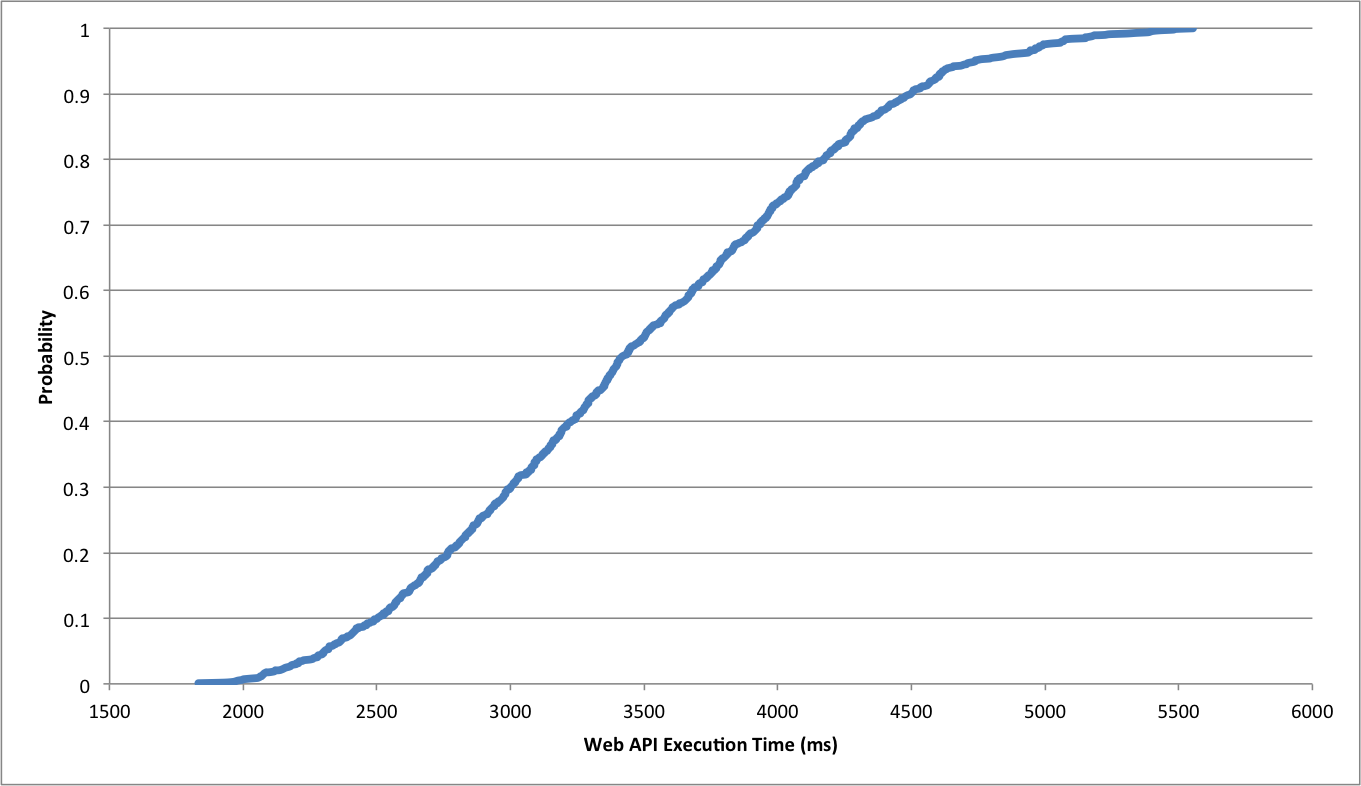
\includegraphics[scale=0.35]{get_all_students_cdf}
\caption{CDF of measured executions times of the StudentInfo\#getAllStudents operation on App Engine.}
\label{fig:get_all_students_cdf}
\vspace{-0.2in}
\end{figure}

Figure~\ref{fig:get_all_students_cdf} shows the empirical cumulative
distribution function (CDF) of measured execution times for the 
StudentInfo\#getAllStudents on
Google App Engine (one of the extreme cases). 
This distribution was obtained by considering the application instrumentation 
results gathered within a window of $1000$ minutes. 
The average of this sample is $3431.79$ms, and the $95^{th}$ percentile
from the CDF is $4739$ms.  Thus, taken as a distribution, the ``spread''
between the average and the $95^{th}$ percentile is more
than $1300$ms.  

% ----- Hiranya: The following observation is wrong. Cerebro spread is 1600ms, not 1100ms -----

%For this case (column 4 in Figure~\ref{fig:diff_summary}), Cerebro's
%spread is approximately $1100$ms.  Thus Cerebro appears to be generating an
%accurate estimate of the $95^{th}$ percentile for this data.  That is, a
%response time SLA of $1100$ms would likely be achievable with probability
%at least $0.95$ 
%for the StudentInfo\#getAllStudents web API when the application is
%running in Google App Engine. 

From this it becomes evident that StudentInfo\#getAll\-Students 
records very high execution times frequently. 
In order to incorporate such high outliers, Cerebro must be conservative 
and predict large values for
the $95^{th}$ percentile. This is a required feature to ensure that 95\% or more 
API invocations have
execution times under the predicted SLA. But as a consequence, the average 
distance between the 
measurements and the predictions increases significantly.

We omit a similar analysis of the other cases in the interest of brevity 
but summarize the tightness results as indicating that Cerebro achieves a
bound that is ``tight'' with respect to the percentiles observed by sampling
the series for long periods. 
%Our analyses with other operations for which
%Cerebro generates conservative bounds have also shown similar results. That is, when the performance of the web API is highly variable and
%when its execution time distribution contains
%many high outliers, Cerebro produces predictions that are less tight. In other words, 
%Cerebro trades off tightness of the predictions for their accuracy.

%\begin{figure}
%\centering
%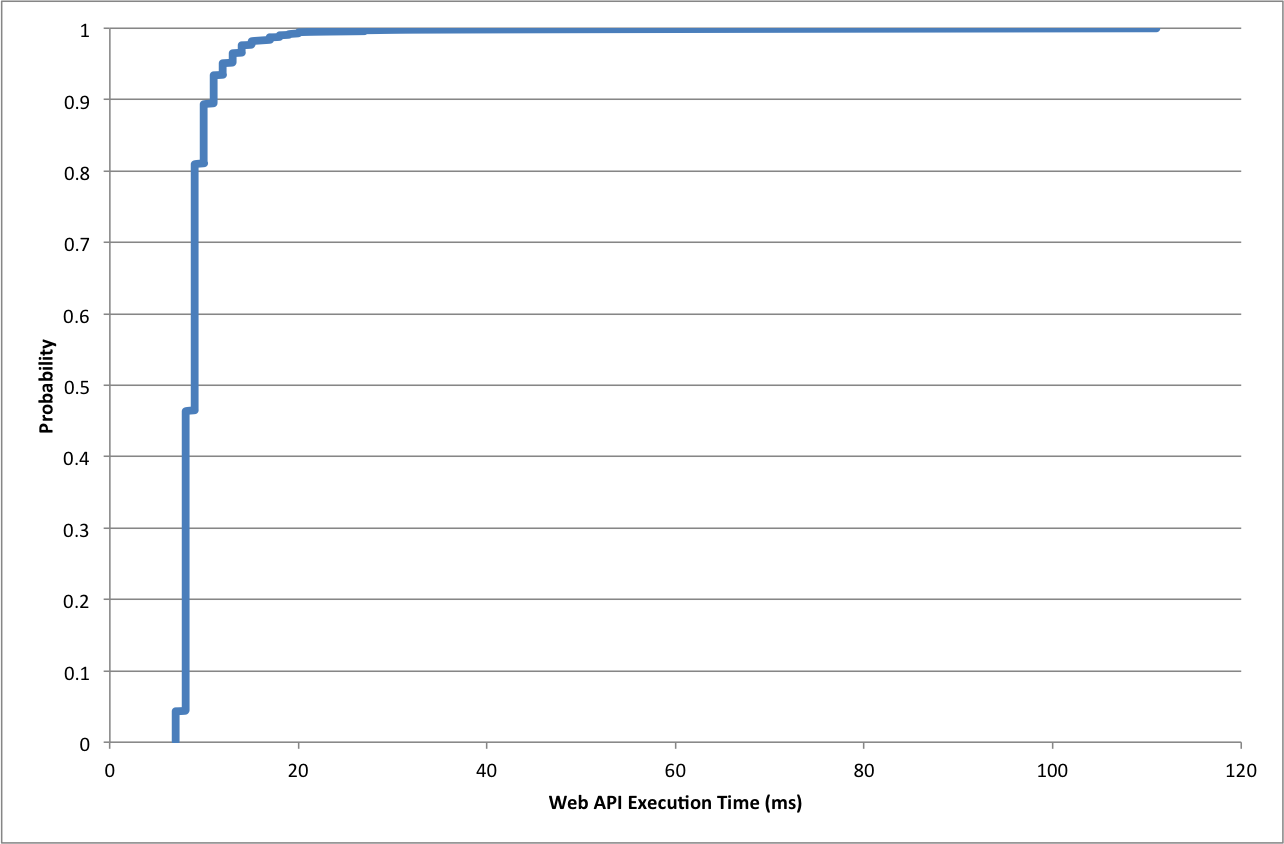
\includegraphics[scale=0.35]{get_student_cdf}
%\caption{CDF of measured response times of the StudentInfo\#getStudent operation on AppScale.}
%\label{fig:get_student_cdf}
%\end{figure}
%
%We also investigate one of the web API operations that result in very tight predictions. 
%Figure~\ref{fig:get_student_cdf} shows the CDF of the measured execution times for the StudentInfo\#getStudent operation on
%AppScale. Again we are considering a sample time frame of 
%$1000$ minutes in the graph.
%This particular distribution has a average of $9.19$ms and a $95^{th}$
%percentile of $12$ms. 
%Given that only 19\% of the values are larger than the mean, 
%and only 2\% of the values are larger than 18ms (twice the mean), 
%we see that this distribution is much more stable and have very few high outliers. This enables Cerebro to generate much
%tighter predictions, without compromising the accuracy of the results. Based on these outcomes we can conclude that Cerebro produces
%very tight upper bound predictions for web APIs whose performance is more stable over time. %For APIs with highly variable performance
%traits resulting in many high outliers, Cerebro generates more conservative and less tight predictions.
%At this point it is worth reaffirming that Cerebro does not consider the actual execution time measurements of the web APIs when
%making SLA predictions for them. It only has access to the cloud SDK benchmarking data gathered by Watchtower. 
%We consider Cerebro's ability to understand the variability of a web API's performance by only looking at the cloud SDK
%benchmarking data, as one of its strengths.

Another interesting observation we can make regarding the tightness of
predictions is that the predictions made in the AppScale cloud platform are
significantly tighter than the ones made in Google App Engine
(Figure~\ref{fig:diff_summary}). 
%Five out of the six scenarios in which Cerebro has generated conservative
%predictions are from App Engine.  Furthermore,
For nine out of the ten operations tested, Cerebro has generated tighter
predictions in the AppScale environment. This is because web API performance
on AppScale is far more stable and predictable thus resulting in fewer
measurements that occur far from the average.

The reason why AppScale's performance is more stable over time is because it is
deployed on a set of closely controlled 
and monitored cluster of virtual machines (VMs) that use a private
Infrastructure-as-a-Service (IaaS) cloud to implement isolation.  In particular, the 
VMs assigned to AppScale do not share nodes with ``noisy neighbors'' in our
test environment.  In contrast, Google App Engine does not expose the
performance characteristics of its multi-tenancy.  While it operates at vastly
greater scale, our test applications also exhibit wider variance of web API
response time when using it.
%We have total control
%over how much resources are assigned to the VMs, and we ensure that they run in total isolation from the other processes 
%running on the underlying hardware.
%This is not the case when running our sample applications on App Engine, where we have no control over 
%the underlying VMs, hardware and the
%scheduling mechanism. Another related, but interesting outcome of these results is that large-scale public cloud platforms like App Engine, while
%highly scalable, may not be able to support tight performance SLAs. Their performance is subject to high variations making it difficult to always support attractive
%performance guarantees. Small private cloud platforms on the other hand can provide much better, consistent and stable performance guarantees, albeit their
%poor scalability. %From an organization's point of view this could be a strong motivator to adopt private cloud over public clouds.
Cerebro, however, is able to predict a correct and tight SLAs for applications
running in either platform: the lower variance private
AppScale PaaS, and the extreme scale but more varying Google App Engine PaaS.

\subsection{Duration of Prediction Validity}

%So far we have examined the accuracy and tightness of the predictions produced by Cerebro. In this section we 
%focus on the validity period of the Cerebro predictions.
%
%Cloud platforms are highly dynamic environments. Some of the changes that may occur in such an environment include:
%\begin{itemize}
%\item addition or removal of hardware resources/VMs/containers,
%\item software updates and upgrades, and
%\item component failures.
%\end{itemize}

%When the platform is subject to such significant and frequent changes, performance SLAs predicted for the web APIs deployed on that
%platform may not hold correct forever. Given enough time the APIs may start violating the predicted SLAs consistently. Therefore, for any
%given SLA prediction we need to have an approximate idea of how long that prediction is going to be valid for. In others words, we need
%to know how long it would take before a predicted SLA value cannot be considered correct. We refer to this time period as the 
%\textit{validity period} of a prediction.

%Ideally we want the validity period of a Cerebro prediction to be infinity. That is, once an SLA prediction has been made for a web API it
%should remain correct forever. If that was the case, the API performance would never degrade to a level where it
%consistently exceeds the originally predicted execution time upper bound. But due to the dynamic nature of the cloud platforms such
%behavior is highly unlikely. From a practical standpoint we can expect the prediction validity period to be some finite duration. 

%We believe
%it is important that cloud administrators be informed about the validity period of predictions so that they can periodically reassess the web
%API SLAs. For example they can run Cerebro periodically (before the prediction validity period expires) on the deployed web APIs to check
%if the predicted execution times have degraded to such a level where they no longer meet the organizational standards for API
%response times. 

To be of practical value to PaaS administration, the duration over which a
Cerebro prediction remains valid must be long enough to allow appropriate
remedial action when load conditions change, and the SLA is in danger of being
violated.  In particular, SLAs must remain correct for at least the time
necessary to allow human responses to changing conditions such as
the commitment of more resources to web APIs that are in violation or alerts
to support staff that customers may be calling to claim SLA breach.  Ideally,
each prediction should persist as correct for several hours or more to match
staff response time to potential SLA violations.

%If that is the case, the cloud administrators can take some remedial actions like 
%committing more resources to the deployed APIs,
%replicating them (horizontal scaling), or notifying the respective API developers about the impending performance issues. However,
%for this to be practical, the validity period of Cerebro predictions should at least be several hours. If the validity period is in the order of minutes,
%a lot of computing time and manpower will be wasted recomputing Cerebro predictions and evaluating the results. Also, given that
%modern cloud platforms are used to host thousands of web APIs, such aggressive re-computation of predictions may not be scalable.

However, determining when a Cerebro-predicted SLA becomes invalid is
potentially complex. For example, given the definition of correctness
described in Subsection~\ref{sec:correctness}, it is possible to report an SLA violation
when the running tabulation of correctness percentage falls below the target
probability (when expressed as a percentage).  However, if this metric is
used, and Cerebro is correct for many consecutive measurements, a sudden
change in conditions that causes the response time to persist at a higher
level will not immediately trigger a violation.  For example, Cerebro might be
correct for several consecutive months and then incorrect for several
consecutive weeks before the overall correctness percentage drops below $95\%$
and a violation is detected.  If the SLA is measured over a year, such time
scales may be acceptable but we believe that PaaS administrators would
consider such a long period of time where the SLAs were continuously in
violation unacceptable.
Thus we propose a more conservative approach to measuring the duration over
which a prediction remains valid than simply measuring the time until the
correctness percentage drops below the SLA-specified value.
%Before we can analyze the validity period of Cerebro predictions, we need to
%develop a model for detecting when a predicted SLA has become invalid. 

Suppose at time $t$ Cerebro predicts value $Q$ as the $p$-th percentile of
some API's execution time.  If $Q$ is a correct and tight prediction,
the probability of API's next measured response time being greater than 
$Q$ is $1-(0.01p)$.  If the time series consists of independent
measurements then the probability of seeing $n$ consecutive values greater
than $Q$ (due to random chance) is $(1-0.01p)^n$. 
For example, using the $95^{th}$ percentile, the probability of seeing $3$
values in a row larger than the actual percentile (purely due to random chance)
is $(0.05)^3 = 0.00012$ or about $1$ in $8333$.

This calculation is conservative with respect to autocorrelation. That is, if
the time series is stationary but autocorrelated, then the number of consecutive 
values above the $95^{th}$ percentile that correspond to a probability of
$0.0012$ is larger than $3$.  For example, in previous
work~\cite{Nurmi:2007:QQB:1791551.1791556} 
using an artificially generated AR(1) series, 
we observed that $5$ consecutive values above the $95^{th}$ percentile
occurred with probability $0.00012$ when the first autocorrelation was $0.5$,
and $14$ when the first autocorrelation was $0.85$.  Thus using an independence
assumption for the series to determine the number of consecutive values above
$Q$ that constitute a ``rare event'' (indicating a possible change in
conditions) is conservative.

In particular, for the $95^{th}$ percentile, we measure the time from when
Cerebro makes a bounds prediction until we observe $n=3$ consecutive
measurement values above that prediction as being the time duration over which
the prediction is valid. We refer to this duration as the \textit{validity duration}.  
Tables~\ref{tab:gae_validity} and~\ref{tab:as_validity} present these durations
for Cerebro predictions in Google App Engine and AppScale
respectively.

%\begin{table}[tdp]
\begin{table}
\caption{Prediction validity period distributions of different operations in
App Engine. Validity durations were computed by observing $3$ consecutive SLA
violations. $5^{th}$ and $95^{th}$ columns represent the 5th and 95th 
percentiles of the
distributions respectively. All values are in hours.
\label{tab:gae_validity}
}
\begin{center}
\begin{tabular}{|c|p{1cm}|p{1cm}|p{1cm}|}
\hline
Operation & $5^{th}$ & Average & $95^{th}$ \\ \hline
StudentInfo\#getStudent & 7.15 & 70.72 & 134.43 \\ \hline
StudentInfo\#deleteStudent & 2.55 & 37.97 & 94.37 \\ \hline
StudentInfo\#addStudent & 1.45 & 26.8 & 64.78 \\ \hline
ServerHealth\#info & 1.41 & 39.22 & 117.71 \\ \hline
Rooms\#getRoomByName & 7.24 & 70.47 & 133.36 \\ \hline
Rooms\#getRoomsInCity & 2.08 & 30.12 & 82.58 \\ \hline
\end{tabular}
\end{center}
\vspace{-0.1in}
\end{table}

\begin{table}
\caption{Prediction validity period distributions of different operations in
AppScale. Validity periods were computed by observing $3$ consecutive SLA
violations. $5^{th}$ and $95^{th}$ 
columns represent the 5th and 95th percentiles of the
distributions respectively. All values are in hours.
\label{tab:as_validity}
}
\begin{center}
\begin{tabular}{|c|p{1cm}|p{1cm}|p{1cm}|}
\hline
Operation & $5^{th}$ & Average & $95^{th}$ \\ \hline
StudentInfo\#getStudent & 6.1 & 60.67 & 115.24 \\ \hline
StudentInfo\#deleteStudent & 6.08 & 60.21 & 114.32 \\ \hline
StudentInfo\#addStudent & 6.1 & 60.67 & 115.24 \\ \hline
ServerHealth\#info & 6.29 & 54.53 & 108.14 \\ \hline
Rooms\#getRoomByName & 6.07 & 59.18 & 112.28 \\ \hline
Rooms\#getRoomsInCity & 1.95 & 33.77 & 84.63 \\ \hline
\end{tabular}
\end{center}
\vspace{-0.2in}
\end{table}

%Next we shall assume that individual SLA
%violations are independent events; i.e. one SLA violation does not depend on
%another SLA violation.  Then, the probability of API violating the predicted
%SLA $n$ times in a row is $(1-0.01p)^n$, if $Q$ is a valid prediction.
%Therefore, if we state that the predicted SLA is invalid after observing $n$
%consecutive violations, the probability of us being correct would be $1 -
%(1-0.01p)^n$. 
%Notice that this value increases with $n$. 

%This implies that we can use consecutive SLA violations made by the API as an indicator of the SLA becoming
%invalid. Larger the number of consecutive violations we observe, more confident we can be about considering the SLA as invalid. 
%Hence for some $n$, if we observe
%the $n$-th consecutive violation at time $t^\prime$, we can consider the duration $t^\prime - t$ as the validity period of the prediction made 
%at time $t$. By the previous argument, the probability of this being an accurate approximation of validity period is $1 - (1-0.01p)^n$.

%Lets consider an example to further clarify this notion. Assume that for some web API at time $t$ Cerebro produces value $Q$ as the 
%prediction of the 95th percentile. Therefore after time $t$, the probability of the API violating this predicted SLA is 0.05, provided
%that $Q$ is a correct prediction. Similarly, if $Q$ is an accurate SLA prediction, and SLA violations are independent events, the probability of the API
%violating the SLA 3 times in a row would be $0.05^3$ or 0.000125. Hence after observing 3 consecutive violations the probability of $Q$
%being an incorrect prediction is $(1 - 0.000125)$ or 0.999875. If we want to be even more confident about detecting invalid SLAs, 
%we can look for an even higher
%number of consecutive SLA violations (i.e. higher $n$).  
%Based on the value they choose for $n$ the validity period of the predictions can be determined
%with a specific level of certainty.

%To evaluate the validity period of Cerebro predictions, we benchmark some of our sample applications for a period of 5 to 6 days on both
%App Engine and AppScale. We also run Watchtower on the same cloud platforms during this period. Then we run Cerebro using
%the Watchtower data to make per-minute SLA predictions (95th percentile; i.e $p=95$) for the entire duration of the tests. Next we choose a sequence of predictions
%in 15 minute intervals. For each of the selected predictions we try to find the time until 3 consecutive violations (i.e $n=3$) by scanning ahead into the trace of
%actual execution times gathered by directly benchmarking the web APIs. This provides us with a distribution of prediction validity periods where
%each validity period has a certainty level of 0.999875.
%However, for some predictions we are not able to find 3 consecutive violations in the traces of actual API execution times. We include
%such cases in the distribution by right censoring. That is, we consider the end of trace as the time to 3 consecutive violations for such cases.

%\begin{figure}
%\centering
%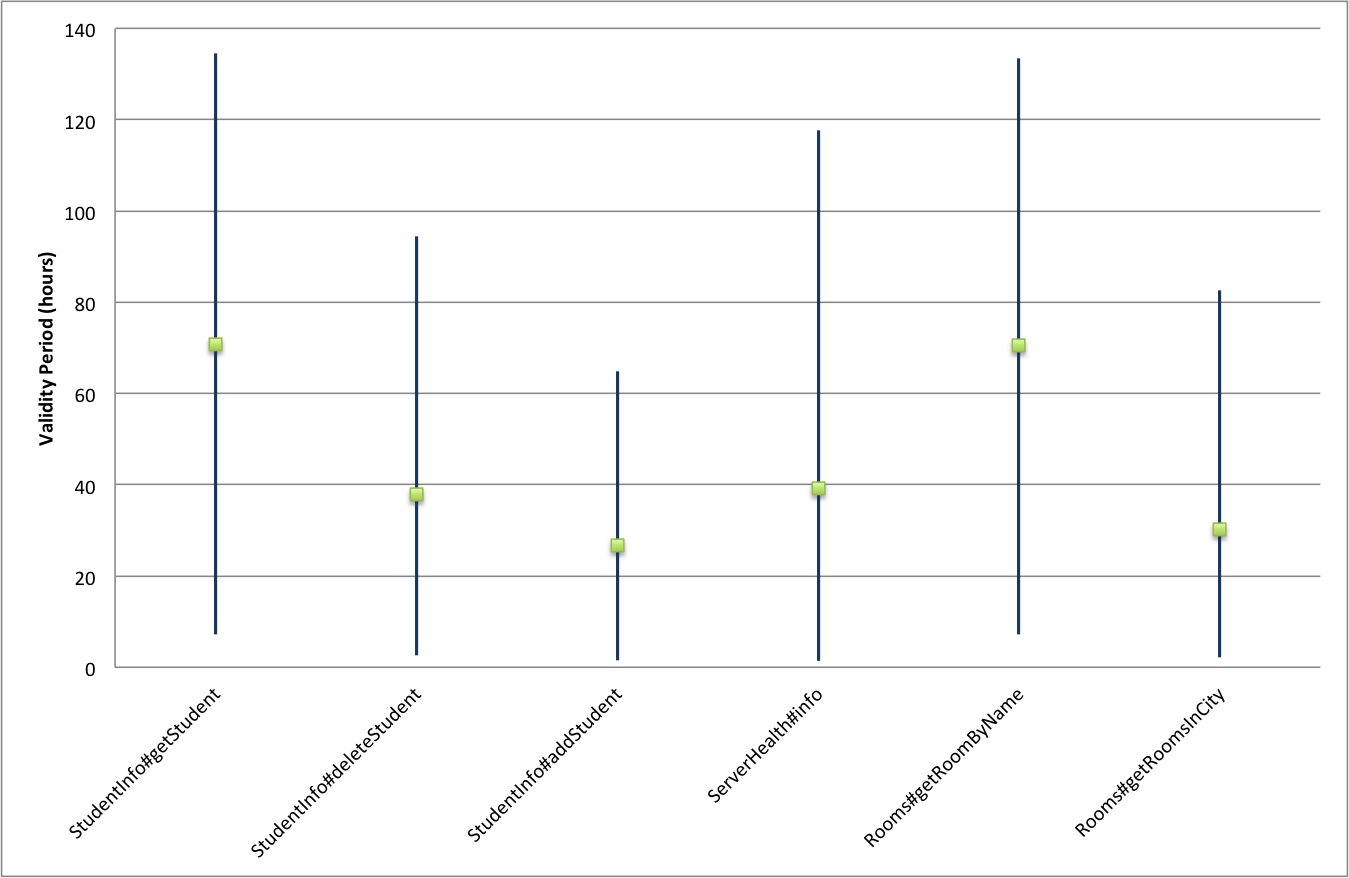
\includegraphics[scale=0.35]{gae_validity}
%\caption{Prediction validity period distributions of different operations in App Engine. The vertical lines indicate the range between the 5th and 95th percentiles of the distributions. The green markers represent the means. Validity periods were computed by observing 3 consecutive SLA
%violations.}
%\label{fig:gae_validity}
%\end{figure}


%\begin{figure}
%\centering
%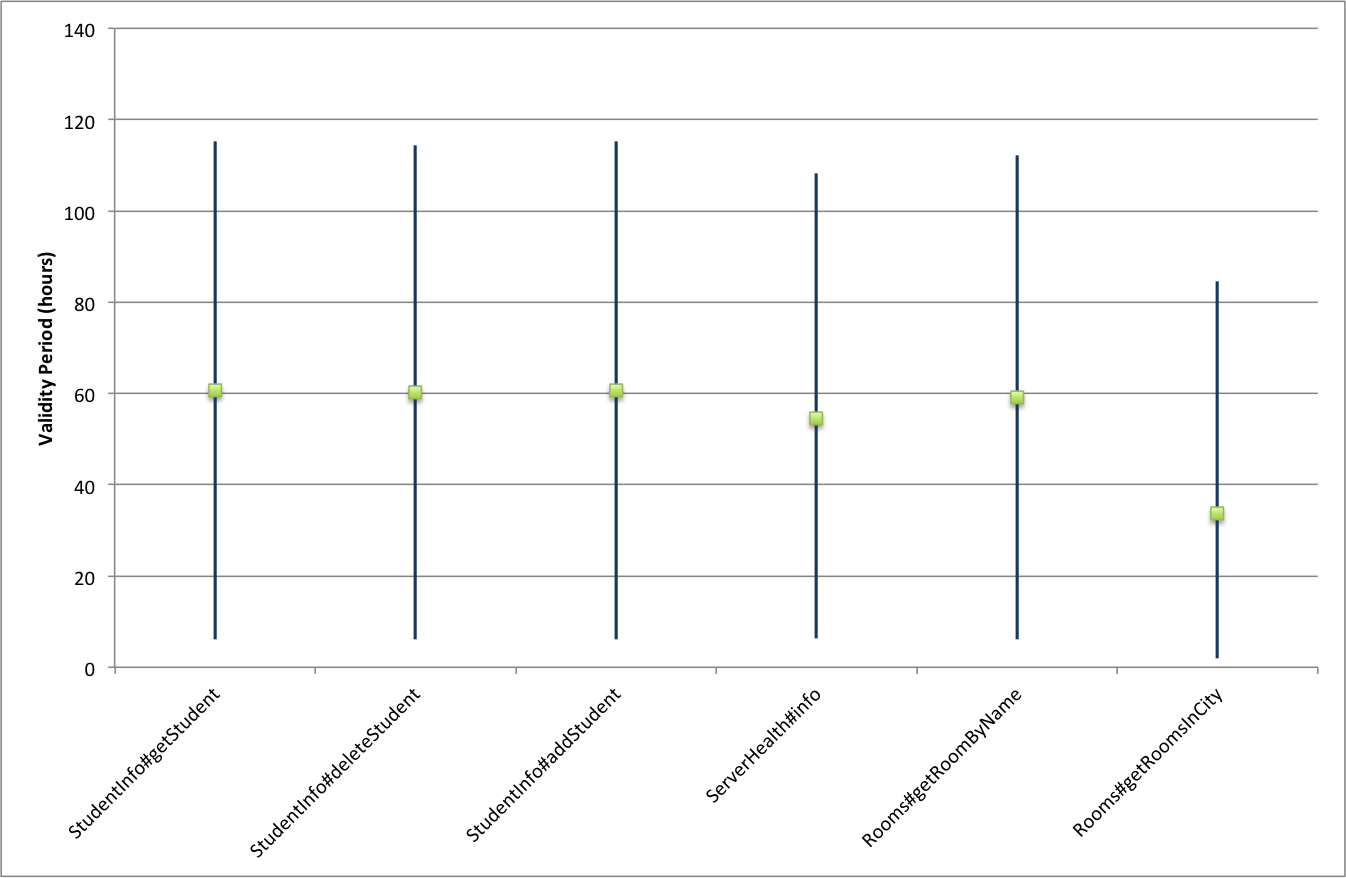
\includegraphics[scale=0.35]{as_validity}
%\caption{Prediction validity period distributions of different operations in AppScale. The vertical lines indicate the range between the 5th and 95th percentiles of the distributions. The green markers represent the means. Validity periods were computed by observing 3 consecutive SLA violations.}
%\label{fig:as_validity}
%\end{figure}

%Table~\ref{tab:gae_validity} shows a summary of the validity period distributions in App Engine. 
%The
%vertical lines represent the range from 5th to 95th percentiles. The square shaped markers on the lines indicate the means of the respective distributions.  
From Table~\ref{tab:gae_validity} 
the average validity duration for all 6 operations considered in App Engine is
longer than $24$ hours. The lowest average value observed is $26.8$ hours, 
and that is for the StudentInfo\#addStudent operation. If we
just consider the $5^{th}$ percentiles of the distributions, they are 
also longer than $1$ hour. The smallest $5^{th}$ percentile value of 
$1.41$ hours is 
given by the ServerHealth\#info operation. This result implies that if we use 
$3$ consecutive violations as a cue for detecting invalid SLAs,
Cerebro predictions made on Google App Engine would be valid for at least
$1.41$ hours or more, at least 95\% of the time.

By comparing the distributions for different operations we can conclude that
API operations that perform a single basic datastore or memcache read tend to
have longer validity durations. In other words, those cloud SDK operations have
fairly stable performance characteristics in Google App Engine. 
This is reflected in
the $5^{th}$ percentiles of StudentInfo\#getStudent and Rooms\#getRoomByName. 
Alternatively
operations that execute writes, iterative reads or long sequences of cloud SDK
operations have shorter prediction validity durations.

For AppScale, 
the smallest average validity period of $33.77$ hours is observed from the
Rooms\#getRoomsInCity operation. All other operations tested in 
AppScale have average prediction validity periods greater
than $54$ hours. The lowest $5^{th}$ percentile value in the 
distributions, which is 1.95 hours, is 
also shown by Rooms\#getRoomsInCity. This means, the SLAs predicted for
AppScale would hold correct for at least $1.95$ hours or more, 
at least 95\% of the time.
%Other operations have 5th percentile values greater than 6 hours. 
The relatively smaller validity period values computed for the
Rooms\#getRoomsInCity operation indicates that the performance of 
iterative datastore reads is subject to some variability 
in AppScale.

%Comparatively, the validity duration recorded in the AppScale
%cloud platform are longer than the ones seen in Google App Engine. 
%
%This is because compared to App Engine our
%test AppScale private cloud is much less dynamic. App Engine is a very large PaaS cloud that is served by thousands of
%nodes possibly distributed over multiple data centers. It is comprised of many components that are not under our control,
%and the entire cloud platform is used by thousands of users worldwide to deploy applications. Such a large scale and
%shared system has to endure a myriad of changes in any given moment (e.g. autoscaling of hardware resources, 
%changing application load, component failures etc.). This behavior affects the performance of the cloud SDK operations, which
%in turns affects the performance SLAs of high-level user code. In contrast, our AppScale
%private cloud is small, deployed on a handful of nodes that are under our control, and during our testing phase it was dedicated
%to running Watchtower and other sample applications. Therefore it is a much more stable environment compared to 
%App Engine -- a fact that is reflected in the calculated prediction validity periods.

\subsection{Learning Duration}
\label{sec:learning}

As described in Subsection~\ref{sec:qbets},
QBETS uses a form of supervised learning internally to determine each of its
bound predictions.  Each time a new prediction is presented, it updates its
internal state with respect to autocorrelation and change-point detection.  As
a result, the correctness percentage may require some number of state updates
to converge to a stable value.

%Earlier we investigated the percentage of measurements that are under predicted SLAs 
%after a fixed amount of time has elapsed.
%In those experiments we made predictions for a fixed-size time period (1000 minutes), 
%and computed the percentage accuracy achieved by Cerebro at the end of the period.
%In this section we are going to analyze the percentage accuracy of Cerebro as a running 
%tabulation. That is, instead of just
%computing the percentage accuracy at the end of 1000 minutes, we are going to compute it 
%for each passing minute. This enables us to
%understand how the percentage accuracy regarding a single web API operation changes over time, 
%and the convergence behavior of Cerebro. We define convergence as the event of Cerebro
%approaching the desired percentage accuracy level (95\% in
%our experiments), and staying close to or above that level consistently.

Figure~\ref{fig:gae_accuracy} shows a running tabulation of
correctness percentage for Cerebro
predictions made in Google App Engine during the first 
$1000$ minutes of operation (one prediction is generated each minute). 
Similarly, in Figure~\ref{fig:as_accuracy} we show a running tabulation of
correctness percentage for Cerebro
predictions made in AppScale during the first 
$1000$ minutes of operation (again, one prediction generated per minute). 

\begin{figure}
\centering
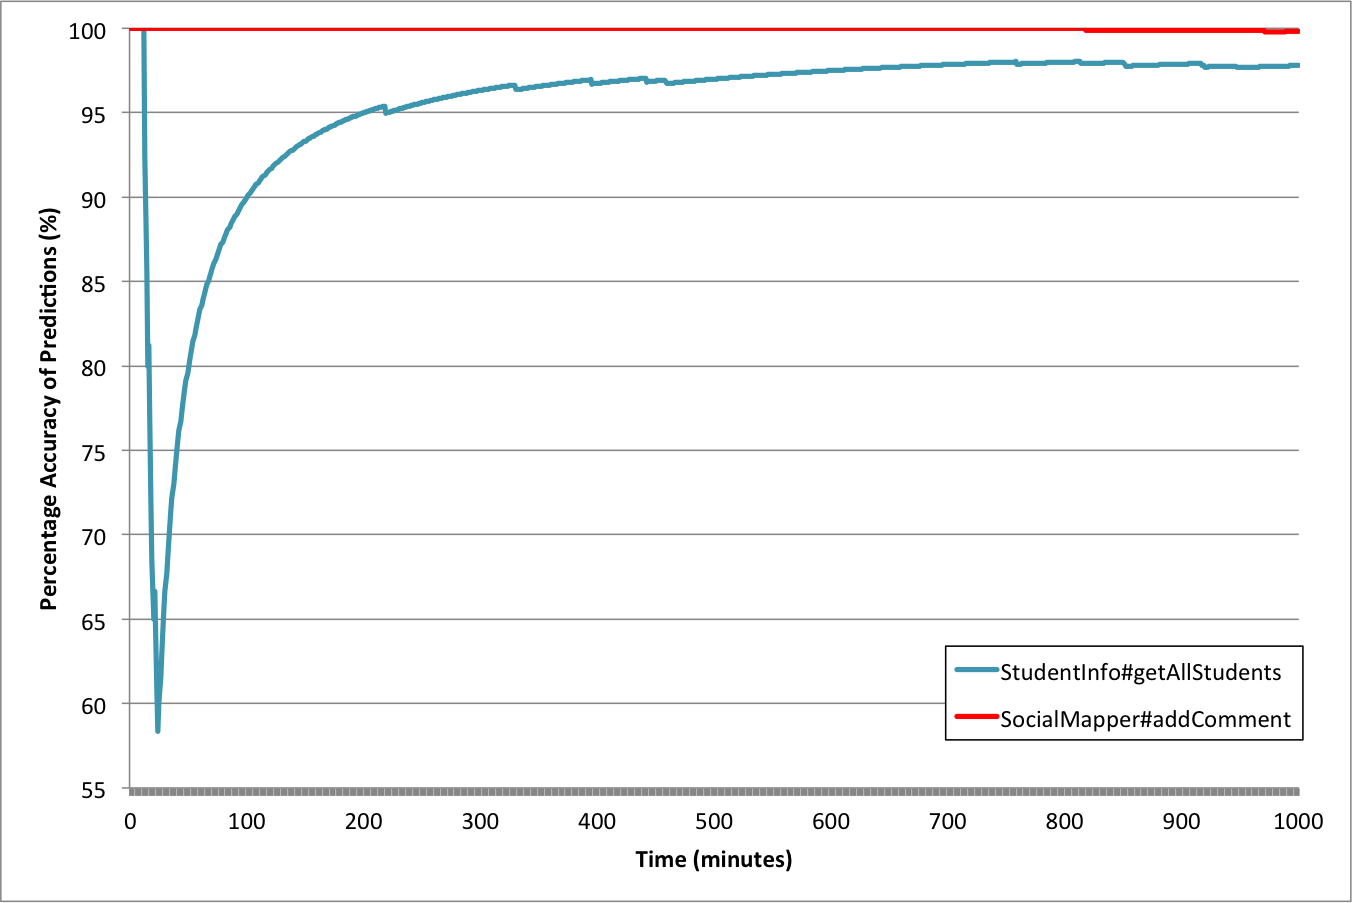
\includegraphics[scale=0.35]{gae_accuracy}
\caption{Running tabulation of correctness percentage for predictions made on Google App 
Engine for first $1000$ minutes, one prediction per minute.}
\label{fig:gae_accuracy}
\vspace{-0.2in}
\end{figure}

\begin{figure}
\centering
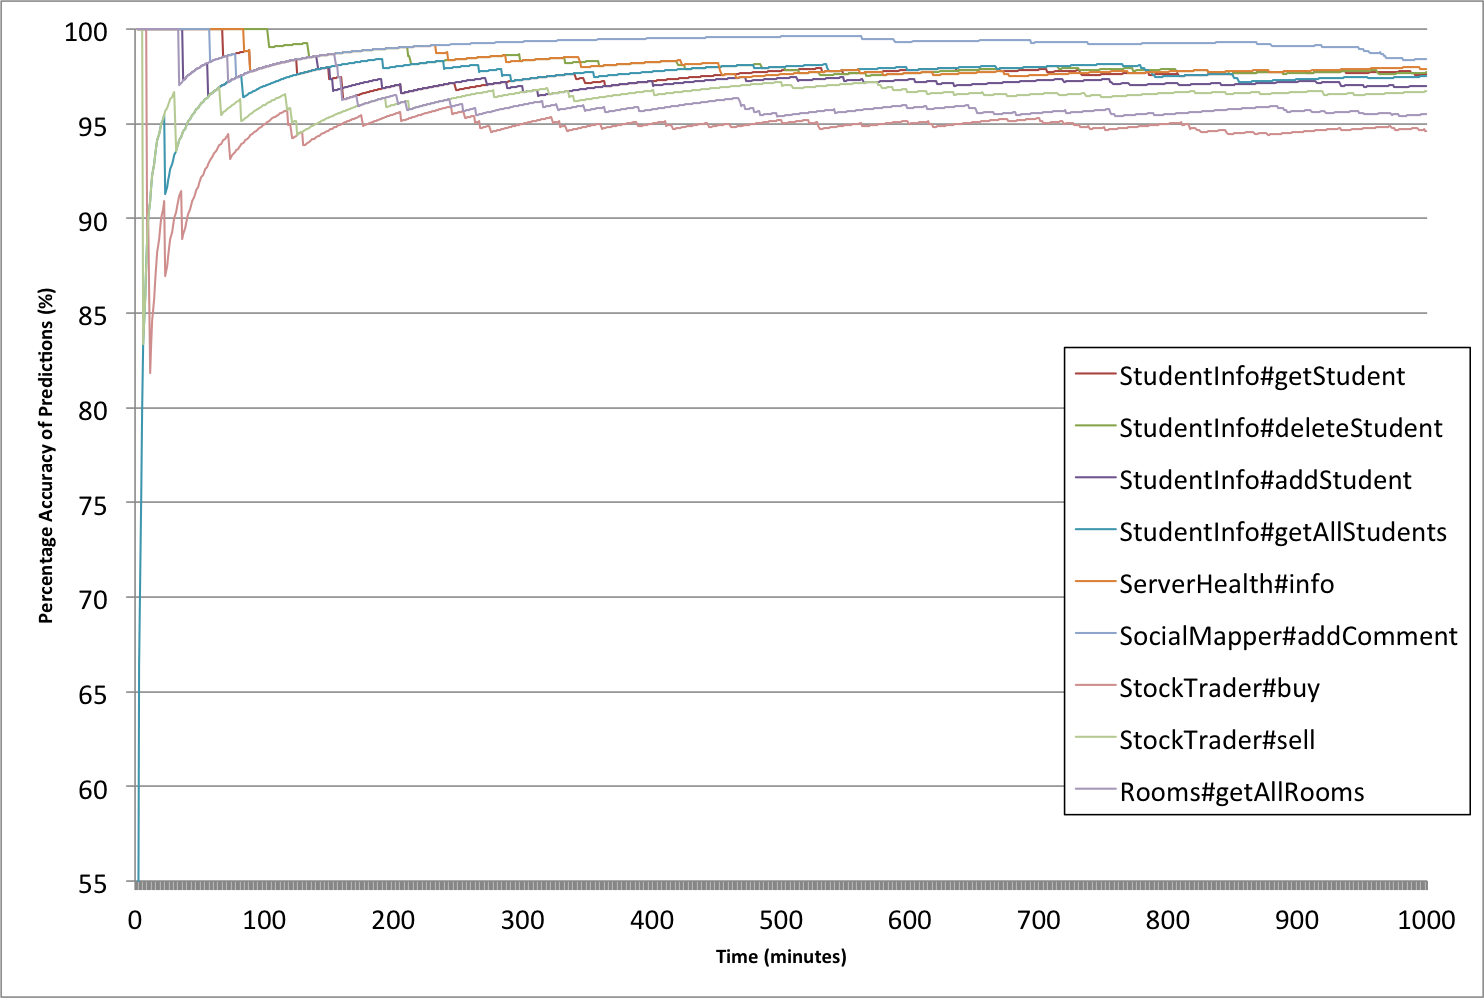
\includegraphics[scale=0.35]{as_accuracy}
\caption{Running tabulation of correctness percentage for predictions made on AppScale for a period
of $1000$ minutes, one prediction per minute.}
\label{fig:as_accuracy}
\vspace{-0.2in}
\end{figure}

For clarity we do not show results for all tested operations. Instead,
we only show data for the operation that reaches stability in the shortest
amount of time, and the operation that takes the longest to converge.
Results for other operations fall between these two extremes.

%As expected, the time series analysis method used by Cerebro (QBETS) takes some time to learn
%from the time series data captured by Watchtower. This is when we see large fluctuations in the percentage accuracy. 
%But once Cerebro has converged it consistently produces highly accurate predictions.
In the worst case, Cerebro takes up to $200$ minutes to 
achieve correctness percentage above $95\%$
in Google App Engine (for StudentInfo\#getAllStudents).
Alternatively, the longest time until Cerebro has ``learned'' the series in
AppScale is approximately $40$ minutes.
%After 275 minutes, we see highly accurate predictions being made on all web API
%operations considered in the tests. After this point, we consistently see percentage accuracy values higher than 96\%. 
%Recall that
%we had configured Cerebro to predict the 95th percentile of the web API executions time. Therefore as long as Cerebro produces
%results with a percentage accuracy close to or higher than 95\%, we can consider the predictions to be correct.
%Figure~\ref{fig:as_accuracy} shows the same results calculated by running Watchtower and the sample applications on AppScale.
%Again we include the results for fastest and slowest convergence only. 
%we can see that Cerebro converges to the preferred percentage accuracy level in 40 minutes at the latest.

%Note that due to the presence of autocorrelation in the series, the
%correctness percentage may drop below its target for some time after it has
%converged.  Especially when the bound is tight, the running tabulation of
%correctness may osscilate slightly above and below the target probability.
%QBETS attempts to adjust for autocorrelation internally but the instantaneous
%correctness percentage at any given moment may be slightly below the target
%value once QBETS has learned the series.  This observation gives further
%credence to the notion that simply observing a correctness percentage below
%the target set for an SLA is not sufficient to determine whether the SLA has
%been violated.

%An interesting observation we can make regarding correctness percentage
%Even after the percentage values have converged, they keep fluctuating 
%around some median value. When the percentage accuracy starts to drop, Cerebro shifts the predictions up thereby increasing
%the percentage accuracy. Similarly when the percentage accuracy increases, Cerebro shifts the predictions down. Due to this
%continuous oscillation, we might encounter instantaneous percentage accuracy values that are slightly 
%below 95\%. This is what is
%happening with respect to the StockTrader\#buy operation in the AppScale environment. Its percentage accuracy converges to a median
%value of 95\% and keeps fluctuating around it. Therefore if we observe the instantaneous percentage accuracy of 
%StockTrader\#buy at any given time, it
%could be slightly above or below 95\%. 
%But as long as this value does not diverge too far from 95\% mark, we can consider Cerebro predictions to
%be accurate.
Summarizing these results, 
the learning time for Cerebro may be several
several hours (up to $200$ minutes in case of 
Google App Engine), before it produces trustworthy and correct 
SLA predictions.  The predictions made during this learning period are not
necessarily incorrect.  It is just not possible to gauge their correctness
quantitatively before the series has been learned.  We envision Cerebro as a
continuous monitoring process in PaaS clouds for which ``startup time'' is not 
an issue.
%Therefore, it is a good idea to start Watchtower in the
%target cloud platform early, and let it run for several hours before allowing API developers to deploy their web APIs on the cloud. 
%Since the
%required warm up period is in hours (as opposed to days or weeks), we believe this is a perfectly viable and reasonable solution to
%ensure that any predictions made by Cerebro are up to the expected standards. 
